\documentclass[11pt]{article}

\usepackage{newtxmath}
\usepackage{fontspec}
\setmainfont{texgyretermes}[Extension=.otf,UprightFont=*-regular,BoldFont=*-bold,ItalicFont=*-italic,BoldItalicFont=*-bolditalic]
\setmonofont{lmmono10}[Extension=.otf,UprightFont=*-regular,Scale=0.95]
\usepackage[margin=1in]{geometry}
\usepackage{microtype}
\usepackage{graphicx}
\usepackage{booktabs}
\usepackage{multirow}
\usepackage{tabularx}
\usepackage{array}
\usepackage{enumitem}
\usepackage{xcolor}
\usepackage{amsmath}
\usepackage[font=small,labelfont=bf]{caption}
\usepackage[authoryear,round]{natbib}
\usepackage{tikz}
\usetikzlibrary{positioning,arrows.meta,fit,calc}
\usepackage{xurl}
\usepackage[colorlinks=true,linkcolor=blue!50!black,citecolor=blue!50!black,urlcolor=blue!50!black]{hyperref}
\usepackage{titlesec}
\usepackage{tcolorbox}
\tcbuselibrary{skins}

\titleformat{\section}{\normalfont\large\bfseries}{\thesection}{0.8em}{}
\titleformat{\subsection}{\normalfont\normalsize\bfseries}{\thesubsection}{0.8em}{}
\titlespacing*{\section}{0pt}{1.4ex plus .5ex}{0.8ex}
\titlespacing*{\subsection}{0pt}{1.1ex plus .4ex}{0.5ex}
\setlist{itemsep=2pt,topsep=3pt}
\renewcommand{\arraystretch}{1.12}

% Generated by analysis/analyze.py. Do not edit.
\newcommand{\QOneMeanF}{16.75}
\newcommand{\QOneMeanU}{14.25}
\newcommand{\QOneMeanDelta}{-2.50}
\newcommand{\QOneClarityDelta}{-2.00}
\newcommand{\QOneUnderDelta}{-0.50}
\newcommand{\QOneNumLower}{4}
\newcommand{\QOneNumTied}{0}
\newcommand{\QOneSignP}{0.0625}
\newcommand{\QOnePermP}{0.0625}
\newcommand{\QOneMinP}{0.0625}
\newcommand{\QOneClarityShare}{80}
\newcommand{\QTwoMeanF}{17.00}
\newcommand{\QTwoMeanU}{16.50}
\newcommand{\QTwoMeanDelta}{-0.50}
\newcommand{\QTwoClarityDelta}{-0.25}
\newcommand{\QTwoUnderDelta}{-0.25}
\newcommand{\QTwoNumLower}{2}
\newcommand{\QTwoNumTied}{2}
\newcommand{\QTwoSignP}{0.25}
\newcommand{\QTwoPermP}{0.25}
\newcommand{\QTwoMinP}{0.0625}
\newcommand{\QTwoClarityShare}{50}
\newcommand{\AllNumLower}{six}
\newcommand{\AllNumTied}{two}
\newcommand{\AllNumHigher}{none}
\newcommand{\NumResponses}{16}
\newcommand{\NumAtCeiling}{16}
\newcommand{\CeilingPoints}{8}
\newcommand{\CeilingShare}{44}
\newcommand{\TotalMax}{18}
\newcommand{\WorstClarityModel}{Llama 3 70B}
\newcommand{\WorstClarityF}{6}
\newcommand{\WorstClarityU}{3}
\newcommand{\PowerNThree}{90}
\newcommand{\PowerNFive}{34}


\newtcolorbox{itembox}[2][]{enhanced,colback=white,colframe=black!45,boxrule=0.5pt,arc=1pt,#1,
  left=5pt,right=5pt,top=4pt,bottom=4pt,fonttitle=\small\bfseries,coltitle=black,
  colbacktitle=black!7,title={#2},fontupper=\small}

\title{\textbf{Effect of Prompt Phrasing on LLMs:\\A Pilot Study of SAT-Style Question Formatting}}
\author{Dylan Santwani\\[2pt]\normalsize Independent researcher}
\date{\normalsize Pilot data collected February 2025 \quad$\cdot$\quad Revised October 2026}

\begin{document}
\maketitle

\begin{abstract}
\noindent
Large language models are trained on web text that contains many standardized-test and textbook problems. I ask whether a question presented in the layout and wording of an SAT item, rather than as a plain paraphrase, changes the quality of a model's worked solution. In a small pilot, four models (GPT-4o, DeepSeek-R1, Qwen2.5 72B and Llama~3 70B) each answered two released SAT items, an algebra word problem and a vocabulary-in-context reading item, once in the original form and once as a plain-prose paraphrase. I scored the \NumResponses{} responses by hand on an \TotalMax-point rubric covering explanation clarity, problem understanding, answer format and correctness. Every response reached the correct answer. On the algebra item all four models scored lower on the paraphrase (mean \QOneMeanF{} to \QOneMeanU{}), and \QOneClarityShare\% of the drop came from clarity. On the reading item the mean fell by 0.5 points and two models did not change. With four paired observations per item, the algebra result is not statistically significant: the exact one-sided $p = \QOnePermP$ is the smallest value four pairs can produce. Several confounds also offer competing explanations, most importantly that the algebra paraphrase changed far more wording than the reading one, that a single scorer knew which version each response came from, and that released SAT items may be memorized. I report the pilot in full with its threats to validity, and I specify a confirmatory study and an evaluation protocol for the question-rewriting pipeline that the hypothesis suggests.
\end{abstract}

\section{Introduction}

A large share of the text that language models learn from is instructional: textbooks, worked examples, practice exams and answer keys. Standardized-test items in particular follow strict writing conventions. A stem states the facts in a fixed order, a single sentence names the quantity to find, and the answer choices are given in a consistent notation. These conventions exist to make questions easier for students to read. If models have seen many questions written this way, a question that follows the conventions may be closer to what the model expects, and the model may reason about it more cleanly.

This paper studies one form of that idea:
\begin{quote}\raggedright
\textbf{Hypothesis.} A question presented in standardized-test form receives a clearer and better-grounded worked solution than the same question presented as a plain paraphrase.
\end{quote}
If the hypothesis holds, it suggests a practical system. A small model could detect questions that need quantitative reasoning and rewrite them into textbook form before a larger model answers them (Section~\ref{sec:application}).

The evidence here is a pilot. It covers two questions, four models and one response per condition, and I scored it myself. A pilot of this size cannot establish the hypothesis, and this revision is written to say so plainly. Its contributions are:
\begin{enumerate}[label=(\arabic*)]
  \item a complete report of the pilot, including the raw scores, the exact prompt, both versions of each question, and corrections to the first version of this paper (Appendix~\ref{app:changes});
  \item an analysis of what the pilot can and cannot support, including exact small-sample tests and the specific confounds that compete with the hypothesis (Sections~\ref{sec:results} and~\ref{sec:discussion});
  \item a confirmatory protocol that separates layout, wording, memorization and input modality, with a sample size that has adequate power (Section~\ref{sec:protocol}); and
  \item a specification of the rewriting pipeline, together with the measurements needed to decide whether it is worth deploying (Section~\ref{sec:application}).
\end{enumerate}

\section{Related work}
\label{sec:related}

\paragraph{Sensitivity to prompt format.}
Model outputs change with features of a prompt that do not change its meaning. \citet{sclar2024quantifying} varied separators, casing and spacing in few-shot prompts and found accuracy differences of up to 76 points on LLaMA-2-13B, and the sensitivity persisted with larger models and instruction tuning. \citet{he2024formatting} rendered the same content as plain text, Markdown, JSON and YAML and found that GPT-3.5-turbo's performance on a code-translation task varied by up to 40\%, while GPT-4 was more robust. \citet{mizrahi2024state} analyzed 6.5 million instances across 20 models and argued that single-prompt benchmark results are brittle and that models should be evaluated over sets of paraphrased instructions. The present study differs in what it varies. Instead of the instruction template or the delimiters, it varies the problem statement itself, contrasting the canonical form of a test item with a paraphrase of it.

\paragraph{Surface form in mathematical reasoning.}
\citet{mirzadeh2024gsmsymbolic} built templated variants of GSM8K problems and found that every model they tested lost accuracy when only the numbers changed. Adding one irrelevant but plausible clause reduced accuracy by up to 65\%. \citet{shi2023distracted} found a similar fragility when irrelevant context is added to arithmetic word problems. Both results show that rewording a quantitative problem can affect performance even when the underlying problem is unchanged. That mechanism is a plausible alternative to the training-distribution explanation proposed here.

\paragraph{Textbook-style training data and contamination.}
\citet{gunasekar2023textbooks} trained phi-1, a 1.3B-parameter code model, mostly on ``textbook quality'' data and reached 50.6\% pass@1 on HumanEval. This is evidence that the style of training data matters, though it concerns training rather than prompting. Standardized-test items also appear in evaluation suites: AGIEval \citep{zhong2023agieval} includes SAT mathematics and English sections. When a released item is in the training data, a model may recall it rather than reason about it. \citet{golchin2024timetravel} detect such contamination by asking a model to complete the beginning of a benchmark instance. \citet{zhang2024gsm1k} built GSM1k, a fresh set of problems matched to GSM8K, and observed accuracy drops of up to 8\% for some model families. Their results showed signs of partial memorization, although frontier models generalized well. For the present question, contamination is a direct confound. A model may do better on the canonical form of a released item because it remembers that item, not because the format helps it reason.

\paragraph{Rewriting inputs before answering.}
The pipeline in Section~\ref{sec:application} is closest to Rephrase and Respond \citep{deng2023rephrase}, in which a model rephrases and expands a question before answering it. Its two-step variant passes the rephrased question from one model to a different responding model. \citet{ma2023query} train a small rewriter with reinforcement learning to adapt queries for a frozen reader model in retrieval-augmented question answering. \citet{zhou2023ape} use a model to search over instructions. The proposal here differs in two ways. The rewrite target is fixed in advance, namely the conventions of standardized-test items, rather than chosen freely by a model. And rewriting is applied only to questions a classifier marks as quantitative. Whether a fixed target does better than unconstrained rephrasing is an empirical question that the protocol in Section~\ref{sec:protocol} is designed to answer. Finally, the pilot's instruction to solve the problem ``in 5 steps'' is a form of chain-of-thought prompting \citep{wei2022cot}, and the protocol's use of a model-based scorer follows the LLM-as-a-judge approach of \citet{zheng2023judging}. That approach reports roughly 80\% agreement with human preferences, but it also documents position, verbosity and self-preference biases that must be controlled.

\section{Pilot study}
\label{sec:method}

\subsection{Models}
Four models were tested in February 2025: GPT-4o \citep{openai2024gpt4o}, DeepSeek-R1 \citep{deepseek2025r1}, Qwen2.5 72B \citep{qwen2024qwen25} and Llama~3 70B \citep{grattafiori2024llama3}. I did not record the access interface, the exact model snapshot or the sampling settings, so the runs cannot be reproduced exactly. Section~\ref{sec:protocol} requires all three to be logged.

\subsection{Items and the paraphrase manipulation}
Two items were taken from released College Board SAT practice materials (Appendix~\ref{app:items}).
\begin{itemize}
  \item \textbf{Q1 (algebra).} A two-step percentage word problem: an item is discounted by 20\%, an 8\% tax is applied, and the student must express the original price in terms of the amount paid, $p$. The correct answer is $p/\bigl((0.8)(1.08)\bigr)$.
  \item \textbf{Q2 (reading).} A vocabulary-in-context sentence completion about particle physicists. The correct answer is \emph{inspecting}.
\end{itemize}
For each item, Gemini produced a version without the standardized-test formatting. I refer to the original as \emph{formatted} and to the rewrite as \emph{unformatted}. The two rewrites differ greatly in how much they change, which matters for interpreting the results (Section~\ref{sec:discussion}):
\begin{itemize}
  \item The Q1 rewrite rewords nearly every clause. It changes \emph{bought} to \emph{was sold to}, \emph{discount} to \emph{reduction}, and \emph{including} to \emph{encompassed}, and it asks for a \emph{formula} instead of an expression. It also drops the answer choices.
  \item The Q2 rewrite keeps the passage almost word for word. It replaces one colon with a period and shortens the question stem, and it keeps the four answer choices.
\end{itemize}
Each version was given to the model as an image. The originals were scans from the test booklet. The rewrites were screenshots of Gemini's output, which appeared as light text on a dark background.

\subsection{Prompt}
Every model received the same instruction, followed by the image:
\begin{quote}\raggedright
\footnotesize\ttfamily Explain your thoughts in solving this question. Solve it in 5 steps, and explain each step. Make your ending answer clear.
\end{quote}
The first version of this paper said that answer choices were withheld from every model. The surviving materials do not support that claim for every condition. The Q2 rewrite contains the choices, and I cannot confirm whether the choices were cropped from the Q1 and Q2 originals. I therefore treat answer-choice visibility as unknown and possibly unequal between conditions.

\subsection{Scoring}
I scored each response by hand on four categories (Table~\ref{tab:rubric}), for a maximum of \TotalMax{} points. All recorded scores are whole numbers. I scored each response knowing which model and which condition it came from, and I did not write descriptions of what each score level means beyond the descriptions in Table~\ref{tab:rubric}.

\begin{table}[t]
\centering\small
\caption{Scoring rubric used in the pilot.}
\label{tab:rubric}
\begin{tabularx}{\linewidth}{@{}l c X@{}}
\toprule
Category & Points & Awarded for \\
\midrule
Clarity & 7 & How clearly each step of the solution is explained. \\
Understanding & 3 & Identifying what the question asks for and how to get there. \\
Format & 3 & Stating the final answer in a form that matches one of the answer choices. \\
Answer & 5 & A correct final answer (5) or an incorrect one (0). \\
\bottomrule
\end{tabularx}
\end{table}

\subsection{Analysis}
The design is paired: each model answered both versions of each item. For each item I report the mean change from formatted to unformatted and the number of models that scored lower. I also report two exact one-sided tests over the four models: a sign test, and a sign-flip permutation test on the mean paired change. With four pairs, the smallest one-sided $p$-value either test can produce is $2^{-4} = \QOneMinP$. Neither test can therefore reach the conventional 0.05 threshold, whatever the data show. I also do not pool the two items into one test, because the hypothesis concerns question types and the pilot contains one question of each type. Statements about a type of question are generalizations from a single item and are labeled as such. All numbers and data figures are generated from \texttt{data/scores.csv} by \texttt{analysis/analyze.py}.

\section{Results}
\label{sec:results}

\begin{table}[t]
\centering\small
\caption{Pilot scores, shown as formatted~/~unformatted. $\Delta$ is the change in total score (unformatted minus formatted).}
\label{tab:scores}
\begin{tabular}{@{}ll cccc c r@{}}
\toprule
Item & Model & Clarity (/7) & Underst.\ (/3) & Format (/3) & Answer (/5) & Total (/18) & $\Delta$ \\
\midrule
\multirow{4}{*}{Q1 (algebra)} & GPT-4o & 6 / 4 & 2 / 2 & 3 / 3 & 5 / 5 & 16 / 14 & $-$2 \\
 & DeepSeek-R1 & 7 / 6 & 1 / 1 & 3 / 3 & 5 / 5 & 16 / 15 & $-$1 \\
 & Qwen2.5 72B & 7 / 5 & 3 / 2 & 3 / 3 & 5 / 5 & 18 / 15 & $-$3 \\
 & Llama 3 70B & 6 / 3 & 3 / 2 & 3 / 3 & 5 / 5 & 17 / 13 & $-$4 \\
\cmidrule(l){2-8} & \textit{Mean} & 6.50 / 4.50 & 2.25 / 1.75 & 3.00 / 3.00 & 5.00 / 5.00 & 16.75 / 14.25 & $-$2.50 \\
\midrule
\multirow{4}{*}{Q2 (reading)} & GPT-4o & 7 / 6 & 3 / 3 & 3 / 3 & 5 / 5 & 18 / 17 & $-$1 \\
 & DeepSeek-R1 & 6 / 6 & 3 / 3 & 3 / 3 & 5 / 5 & 17 / 17 & 0 \\
 & Qwen2.5 72B & 6 / 6 & 3 / 2 & 3 / 3 & 5 / 5 & 17 / 16 & $-$1 \\
 & Llama 3 70B & 6 / 6 & 2 / 2 & 3 / 3 & 5 / 5 & 16 / 16 & 0 \\
\cmidrule(l){2-8} & \textit{Mean} & 6.25 / 6.00 & 2.75 / 2.50 & 3.00 / 3.00 & 5.00 / 5.00 & 17.00 / 16.50 & $-$0.50 \\
\bottomrule
\end{tabular}

\end{table}

\begin{figure}[t]
\centering
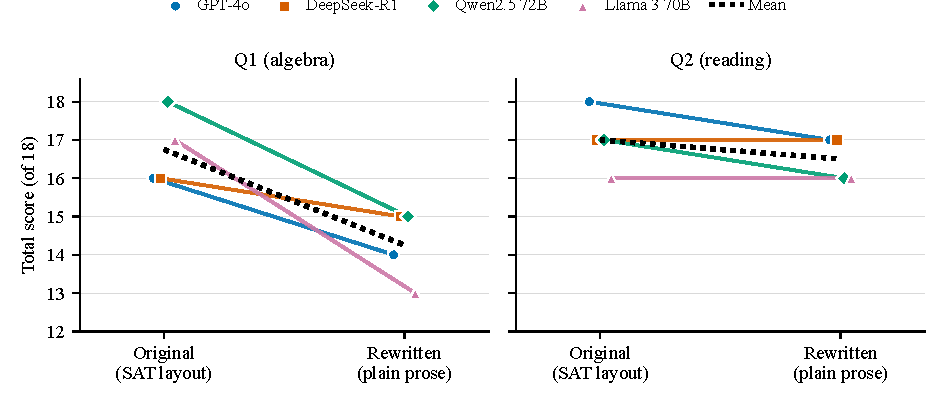
\includegraphics[width=\linewidth]{figures/paired-totals.pdf}
\caption{Total score for each model on the original and rewritten version of each item. Lines connect the same model. The dotted black line connects the means. Points are offset horizontally so that tied scores remain visible.}
\label{fig:paired}
\end{figure}

\begin{figure}[t]
\centering
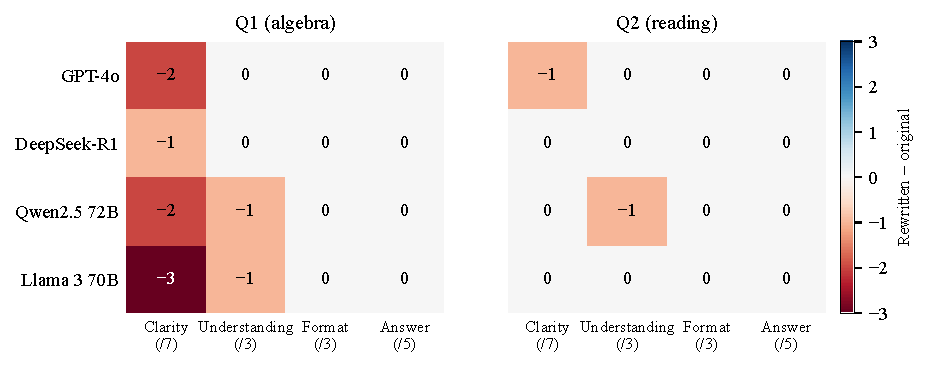
\includegraphics[width=0.94\linewidth]{figures/category-deltas.pdf}
\caption{Change in each rubric category (rewritten minus original) by model. Format and Answer did not change for any model because every response received full marks in both.}
\label{fig:deltas}
\end{figure}

Table~\ref{tab:scores} gives every score, Figure~\ref{fig:paired} shows the paired totals, and Figure~\ref{fig:deltas} breaks the change down by category.

\paragraph{Correctness and format were at the ceiling.} All \NumResponses{} responses reached the correct answer and stated it in the expected form. These two categories make up \CeilingPoints{} of the \TotalMax{} points (\CeilingShare\%) and did not vary at all. Every difference observed in the pilot therefore comes from the two judgment-based categories, clarity and understanding. The pilot gives no evidence about whether formatting affects whether a model gets the answer right.

\paragraph{Q1 (algebra).} All four models scored lower on the rewrite. The mean total fell from \QOneMeanF{} to \QOneMeanU{} ($\Delta = \QOneMeanDelta$), and \QOneClarityShare\% of that change was in clarity (mean $\Delta = \QOneClarityDelta$). The largest single change was \WorstClarityModel's clarity, which fell from \WorstClarityF{} to \WorstClarityU{}. Understanding fell by one point for Qwen2.5 72B and Llama~3 70B and was unchanged for GPT-4o and DeepSeek-R1. Because the direction was the same for all four models, both exact tests return $p = \QOneSignP$. That is the smallest value attainable with four pairs, and it is not significant at $\alpha = 0.05$.

\paragraph{Q2 (reading).} The mean total fell from \QTwoMeanF{} to \QTwoMeanU{} ($\Delta = \QTwoMeanDelta$). GPT-4o lost one point of clarity and Qwen2.5 72B lost one point of understanding; DeepSeek-R1 and Llama~3 70B did not change. The sign test, computed over the two models whose scores changed, gives $p = \QTwoSignP$.

\paragraph{Across items.} Of the eight model--item pairs, \AllNumLower{} scored lower on the rewrite, \AllNumTied{} were tied and \AllNumHigher{} scored higher.

\section{Discussion}
\label{sec:discussion}

The pattern is consistent with the hypothesis. Every change went in the predicted direction, and the larger change occurred on the quantitative item. However, at least six other explanations fit the same data, and the pilot cannot tell them apart.

\begin{enumerate}[label=\textbf{T\arabic*.},leftmargin=2.2em]
  \item \textbf{Unequal manipulation strength.} The Q1 rewrite changed nearly every clause, while the Q2 rewrite changed one punctuation mark and the question stem. The larger effect on Q1 may reflect a larger change to Q1 rather than a difference between algebra and reading questions. This is the most serious problem for the claim that formatting matters more for quantitative questions.
  \item \textbf{Wording, not format.} The Q1 rewrite introduced less common phrasing (\emph{encompassed}, \emph{denoted as}) and changed the requested object from an expression to a formula. The drop may come from harder or less precise language. In that case the effect would be a cost of this particular paraphrase rather than a benefit of SAT layout, which is the kind of surface-form sensitivity documented by \citet{mirzadeh2024gsmsymbolic} and \citet{shi2023distracted}.
  \item \textbf{Image rendering.} Originals were printed scans; rewrites were dark-mode screenshots. Differences in how the vision encoder reads each image are confounded with the manipulation.
  \item \textbf{Answer-choice visibility.} Whether choices were visible may have differed between conditions (Section~\ref{sec:method}), and visible choices change both the task and the Format category.
  \item \textbf{Memorization.} Both items are released SAT questions that may appear in training data. A model may produce a cleaner solution to an item it has seen before \citep{golchin2024timetravel,zhang2024gsm1k}. That would make the effect contamination, not format.
  \item \textbf{Scorer expectation.} One scorer, who held the hypothesis and knew each response's condition, assigned every score. Clarity, the category that carried most of the effect, is also the most subjective, and no score-level descriptions were written in advance.
\end{enumerate}

In addition, the pilot has one response per condition with unrecorded sampling settings, so ordinary run-to-run variation is unmeasured. A one- or two-point difference on a seven-point clarity scale could be within that variation.

The defensible reading is therefore narrow. In this pilot, a heavily reworded algebra item received less clear explanations from all four models, and a lightly reworded reading item barely changed. That is enough to justify a properly controlled study. It is not evidence that textbook formatting improves reasoning in general.

\section{Proposed confirmatory study}
\label{sec:protocol}

The design below addresses T1--T6 directly and makes items, rather than models, the unit of replication.

\paragraph{Items.} Use the SAT-Math (220 items) and SAT-English (206 items) sections of AGIEval \citep{zhong2023agieval}, which are public and widely used, plus a new set of at least 40 items I write myself in SAT style and have never published. The new items are the control for memorization (T5).

\paragraph{Conditions.} Each item appears in five forms, with text input unless stated otherwise:
\begin{itemize}
  \item[C0] the original item as text;
  \item[C1] the same words with the layout removed: no item number, choices folded into the sentence, and no line breaks (layout only);
  \item[C2] a meaning-preserving paraphrase, checked by a second reader for equivalence and matched to the original for length and reading level (wording only);
  \item[C3] a deliberately non-canonical paraphrase in conversational style (wording and register);
  \item[C4] C0 rendered as an image in a fixed, matched style (modality only; addresses T3).
\end{itemize}
Every condition is run once with answer choices and once without, and the setting is recorded (T4). Comparing C0 with C1 isolates layout and comparing C0 with C2 isolates wording, which addresses T1 and T2. Using the same paraphrasing procedure for every item also fixes T1.

\paragraph{Models and sampling.} Include the four pilot models, current open-weight models, and small (3B--8B) models whose accuracy on these items is below the ceiling, so that the correctness category can vary. Each item and condition is sampled five times at a fixed temperature, with the exact model identifier, access interface, date and all decoding parameters logged.

\paragraph{Scoring.} Correctness is scored automatically. Clarity and understanding are scored with a rubric that includes a written example for every score level. Scorers see responses in random order without the condition label, and anything that identifies the condition (such as quoted question text) is removed before scoring. Two human raters score a stratified subset of at least 200 responses, and agreement is reported as a quadratic-weighted $\kappa$. A model judge scores the full set, and its agreement with the human raters is reported on that subset. The judge is not one of the models under test, and it scores each response in two presentation orders to control the biases documented by \citet{zheng2023judging} (T6).

\paragraph{Analysis.} The primary outcomes are accuracy and rubric score. They are fitted with mixed-effects models (logistic and linear, respectively) that have a fixed effect for condition, its interaction with subject (math or English) and with item novelty (released or new), and random intercepts for item and model. The hypotheses and the analysis are registered before any data are collected. As a check on sample size: when items are the unit of analysis, a two-sided paired test at $\alpha = 0.05$ has 80\% power with \PowerNFive{} items for a standardized effect of $d_z = 0.5$, and with \PowerNThree{} items for $d_z = 0.3$. The planned sets exceed both.

\section{The rewriting pipeline}
\label{sec:application}

\begin{figure}[t]
\centering
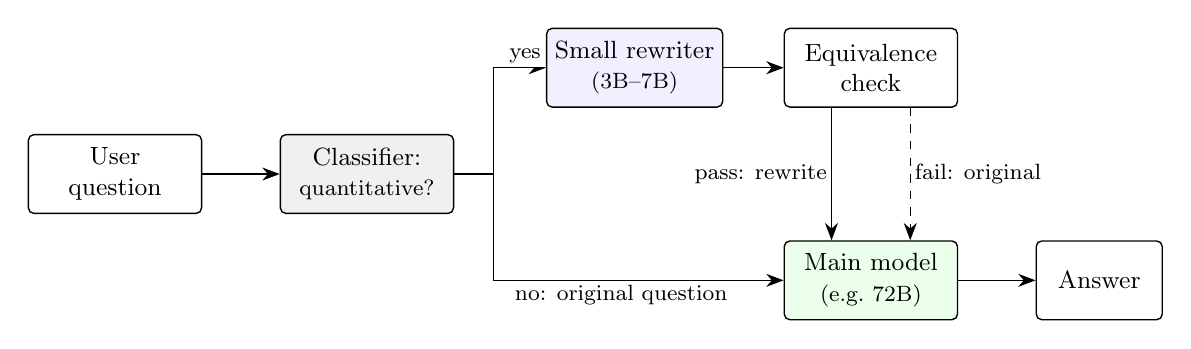
\begin{tikzpicture}[
  box/.style={draw, rounded corners=2pt, align=center, font=\small, minimum height=10mm, minimum width=22mm, inner sep=3pt, line width=0.5pt},
  small/.style={box, fill=blue!6},
  large/.style={box, fill=green!8},
  dec/.style={box, fill=black!6},
  lab/.style={font=\footnotesize, fill=white, inner sep=1.5pt},
  >={Stealth[length=2.2mm]}
]
\node[box]               (user) at (0,0)      {User\\question};
\node[dec]               (cls)  at (3.2,0)    {Classifier:\\\footnotesize quantitative?};
\node[small]             (rw)   at (6.6,1.35) {Small rewriter\\\footnotesize (3B--7B)};
\node[box]               (chk)  at (9.6,1.35) {Equivalence\\check};
\node[large]             (main) at (9.6,-1.35){Main model\\\footnotesize (e.g.\ 72B)};
\node[box,minimum width=16mm] (ans) at (12.5,-1.35) {Answer};
\draw[->] (user) -- (cls);
\draw[->] (cls.east) -- ++(0.5,0) |- node[lab,pos=0.8,above]{yes} (rw.west);
\draw[->] (cls.east) -- ++(0.5,0) |- node[lab,pos=0.72,below]{no: original question} (main.west);
\draw[->] (rw) -- (chk);
\draw[->] ([xshift=-5mm]chk.south) -- node[lab,left]{pass: rewrite} ([xshift=-5mm]main.north);
\draw[->,dashed] ([xshift=5mm]chk.south) -- node[lab,right]{fail: original} ([xshift=5mm]main.north);
\draw[->] (main) -- (ans);
\end{tikzpicture}
\caption{Proposed pipeline. Questions that the classifier marks as quantitative are rewritten into standardized-test form by a small model. A rewrite is used only if it passes an equivalence check; otherwise the main model receives the original question.}
\label{fig:pipeline}
\end{figure}

Figure~\ref{fig:pipeline} shows the system the hypothesis suggests. A lightweight classifier decides whether a question needs quantitative reasoning. If it does, a small model rewrites the question into standardized-test form: facts in order, one explicit target quantity, and consistent notation. The main model then answers the rewrite. This revision adds an equivalence check that was not in the original design. Rewriting can change a problem's meaning, which was already a concern for Q2 in the pilot, and a rewrite that changes the meaning can turn a correct answer into a wrong one.

The pipeline is worth building only if it beats simpler alternatives. Its evaluation should compare it with four baselines: no rewriting, Rephrase and Respond with the main model rephrasing \citep{deng2023rephrase}, unconstrained rephrasing by the same small model, and rewriting every question regardless of type. Five quantities should be reported:
\begin{itemize}
  \item the change in accuracy and rubric score on quantitative questions;
  \item the change on non-quantitative questions that the classifier wrongly sends to the rewriter;
  \item the rate at which rewrites fail the equivalence check, and the rate at which they change the correct answer;
  \item the added latency and cost per question; and
  \item the classifier's precision and recall.
\end{itemize}
The confirmatory study answers the prior question. If C0 does not beat C2 for quantitative items, a fixed textbook-style target has no advantage, and any benefit of rewriting would have to come from elsewhere.

\section{Limitations}
The pilot's limits are discussed in Section~\ref{sec:discussion}: two items, four models, one sample per condition, unrecorded model versions and settings, a single scorer who knew each condition, ceiling effects, and confounds of wording, rendering, answer choices and memorization. The confirmatory design has limits of its own. AGIEval items are themselves likely to be in training data, which is why the newly written items are needed. SAT conventions are only one textbook register. And a rubric score for clarity, even with blind scoring and measured agreement, measures how an explanation reads rather than whether the reasoning behind it is sound.

\section{Conclusion}
In a two-item pilot, all four models gave less clear explanations of an algebra problem after it was reworded out of SAT form, while a lightly edited reading item barely changed. Every response was correct, so the effect is on the explanations and not on accuracy. The result fits the hypothesis that the canonical test form helps models reason, but it fits several duller explanations equally well, and four paired observations cannot reach statistical significance. The useful outcome of the pilot is a sharper question and a design that can answer it: separate layout from wording, control for memorization, score blind, and test enough items to detect a modest effect. Only if that study finds an effect of the canonical form on quantitative items is the rewriting pipeline worth building.

\paragraph{Data and code.} Scores, analysis code and figure sources are available at \url{https://github.com/dylansantwani/prompt-phrasing-llms}. The original February 2025 version of this paper is preserved in \texttt{v1/}.

\bibliographystyle{plainnat}
\bibliography{refs}

\clearpage
\appendix
\section{Items}
\label{app:items}

The items are reproduced from released College Board SAT practice materials for the purpose of analysis. The rewrites are transcribed from the Gemini output used in the pilot.

\vspace{4pt}
\noindent\begin{minipage}[t]{0.485\linewidth}
\begin{itembox}[equal height group=q1]{Q1, formatted (original)}
Alma bought a laptop computer at a store that gave a 20 percent discount off its original price. The total amount she paid to the cashier was $p$ dollars, including an 8 percent sales tax on the discounted price. Which of the following represents the original price of the computer in terms of $p$?\par\smallskip
\begin{tabular}{@{}l@{\hspace{2.2em}}l@{}}
A)~$0.88p$ & B)~$\dfrac{p}{0.88}$\\[8pt]
C)~$(0.8)(1.08)p$ & D)~$\dfrac{p}{(0.8)(1.08)}$
\end{tabular}
\end{itembox}
\end{minipage}\hfill
\begin{minipage}[t]{0.485\linewidth}
\begin{itembox}[equal height group=q1]{Q1, unformatted (Gemini rewrite)}
A laptop computer was sold to Alma at a store with a 20\% reduction from its regular price. The total cost Alma paid, denoted as $p$ dollars, encompassed an 8\% sales tax calculated on the reduced price. Which of the following formulas calculates the original price of the laptop using $p$?
\end{itembox}
\end{minipage}

\vspace{6pt}
\noindent\begin{minipage}[t]{0.485\linewidth}
\begin{itembox}[equal height group=q2]{Q2, formatted (original)}
Particle physicists like Ayana Holloway Arce and Aida El-Khadra spend much of their time \underline{\hspace{1.4em}} what is invisible to the naked eye: using sophisticated technology, they closely examine the behavior of subatomic particles, the smallest detectable parts of matter.\par\smallskip
Which choice completes the text with the most logical and precise word or phrase?\par\smallskip
\begin{tabular}{@{}l@{\hspace{2.2em}}l@{}}A)~selecting & B)~inspecting\\ C)~creating & D)~deciding\end{tabular}
\end{itembox}
\end{minipage}\hfill
\begin{minipage}[t]{0.485\linewidth}
\begin{itembox}[equal height group=q2]{Q2, unformatted (Gemini rewrite)}
Particle physicists like Ayana Holloway Arce and Aida El-Khadra spend much of their time \underline{\hspace{1.4em}} what is invisible to the naked eye. Using sophisticated technology, they closely examine the behavior of subatomic particles, the smallest detectable parts of matter.\par\smallskip
Which word or phrase best completes the sentence?\par\smallskip
\begin{tabular}{@{}l@{\hspace{2.2em}}l@{}}A)~selecting & B)~inspecting\\ C)~creating & D)~deciding\end{tabular}
\end{itembox}
\end{minipage}

\section{Changes from the first version}
\label{app:changes}
The first version (February 2025, preserved in \texttt{v1/}) differs from this one in the following ways.
\begin{itemize}
  \item \textbf{Score scale.} It stated that scores were out of 15 in 0.1 increments. The rubric sums to 18 and every recorded score is a whole number; this version uses 18.
  \item \textbf{Model label.} One chart labeled the Qwen model as Qwen2.5 14B. Every Qwen response came from Qwen2.5 72B; the label was a typo. DeepSeek is identified here as DeepSeek-R1.
  \item \textbf{Answer choices.} It stated that no model saw answer choices. The archived Q2 rewrite contains them and the cropping of the originals cannot be confirmed, so this version treats choice visibility as unknown.
  \item \textbf{Strength of claims.} It described the Q1 change as significant and concluded that rewriting \emph{could produce more accurate results}. Accuracy did not vary in the pilot, and the change is not statistically significant; both claims are withdrawn.
  \item \textbf{Terminology.} ``Logistical reasoning'' is replaced by ``quantitative reasoning''. The reference to ``close clones of GPT-2'' is removed.
  \item \textbf{Additions.} Related work, exact tests, threats to validity, the confirmatory protocol, the equivalence check in the pipeline, and reproducible figures generated from the data.
\end{itemize}

\end{document}
